\chapter*{Introduction}
\addcontentsline{toc}{chapter}{Introduction}
	Ce document a pour objectif de présenter la conception de l'application MyCalendar. Cette application, écrite en C++ avec le framework Qt4, présente une interface graphique correspondant à un emploi du temps semaine par semaine modifiable localement. L'utilisateur peut s'il le souhaite créer, modifier, ou supprimer des évènements.

	Autour de ces fonctionnalités basiques s'attachent deux autres fonctionnalités permettant à l'utilisateur d'intéragir avec certains services en ligne pour importer ou exporter des évènements depuis Internet vers l'application locale et vice-versa.\\

	Petit rappel des spécifications des exigences logicielles à partir desquelles la présente conception est basée :
	\begin{itemize}
		\item Architecture modulaire permettant une maintenance facile de l'application ;
		\item Interface graphique (GUI\footnote{Graphical User Interface}) \emph{user-friendly} par semaine ;
		\item Respect de la charte graphique GNU/Linux ;
		\item Édition locale de l'emploi du temps (ajout, modification, suppression) par clics intuitifs sur la GUI ;
		\item Gestion des conflits (que faire lorsque l'utilisateur essaie d'ajouter un évènement sur un créneau non libre ?) ;
		\item Sauvegarde locale des évènements ;
		\item Exporter l'emploi du temps vers un service en ligne ;
		\item Récupérer l'emploi du temps depuis ce même service en ligne ;
		\item Protection de l'emploi du temps distant avec des identifiants de connexion ;
		\item Utilisation du protocole REST pour la communication avec ce service en ligne ;
		\item Communication non bloquante et temps de réponse de l'ordre de la seconde ;
	\end{itemize}
	\vspace{0.5cm} 
	Une autre exigence est concernée par la conception de l'application puisque nous avons eu le temps de l'implémenter : la récupération d'un emploi du temps universitaire depuis le site de gestion d'emploi du temps de l'Université de Nantes. Cependant, aucun autre format d'emploi du temps n'a été supporté, cette exigence ayant été elle aussi reportée.
		

\chapter{Conception générale}
	%GUILLAUME
	Afin de répondre à la première exigence, c'est-à-dire concevoir l'application à partir d'une architecture modulaire, nous avons utilisé le pattern architectural MVC (pour Model-View-Controller). Cette architecture nous permet de diviser l'application en plusieurs sous-systèmes :
	\begin{enumerate}
		\item L'interface graphique utilisateur ;
		\item Le modèle, contenant tous les évènements et proposant des méthodes pour agir dessus ;
		\item Les interfaces de communication, pour interagir avec différents services d'emploi du temps en ligne ;
	\end{enumerate}
	Le contrôleur joue quant à lui le rôle d'arbitre entre tous ces systèmes.\\
	Exemples :
	
	La vue demande la sauvegarde des évènements dans un fichier local : le contrôleur reçoit le signal correspondant et traite la demande.
	
	La vue demande l'export des évènements vers un service en ligne : le contrôleur reçoit ce signal, vérifie la connexion à ce service (est-ce que l'utilisateur est authentifié ?) et appelle la bonne interface de communication.
	
	Un conflit est détecté lors de l'ajout d'un nouvel évènement : le contrôleur traite ce conflit, soit en demandant à l'utilisateur que faire, soit en appliquant un comportement par défaut par exemple.\\
	
	Ci-dessus, un diagramme de classe généraliste présentant ce système dans sa globalité. La conception de chaque sous-système est présentée dans les prochains chapitres.
	\begin{figure}
		\centering
		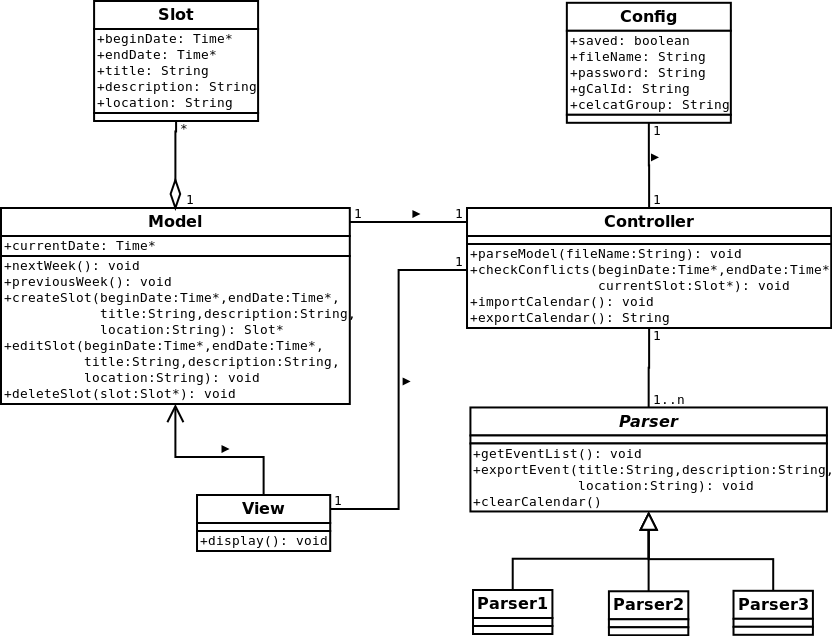
\includegraphics[scale=0.55]{DiagrammeGL.png}
		\caption{Diagramme de classe général}
	\end{figure}
	\FloatBarrier

\chapter{Conception du modèle}
	%JEROME
	
	Le modèle contient toutes les données de l'application, aussi bien les objets de l'emploi du temps manipulés utilisés par les différentes classes que la configuration du logiciel. Il correspond à la première partie du patron architectural MVC. 
	
	Le modèle est composé des classes suivantes :
	%Insérer ici le diagramme de classe du modèle
	
	\section La classe Modèle
	La classe modèle est la classe principale de ce sous-système. Elle possède plusieurs types d'attributs :
	\begin{itemize}
		\item Time* currentDate : un pointeur vers un objet de type Time qui contient la date courante.
        \item Set<Slot*> slotlist : un ensemble de pointeurs de slot contenu dans un Set afin de trier les objets. De cette manière, les opérations de base (ajout, suppression, lecture et mise à jour) sont disponibles facilement, en parcourant la liste via un itérateur. Pour cela, il sera convenu de définir une méthode de comparaison des créneaux qui se basera sur leur date de début pour effectuer ce tri.
	\end{itemize}
	
	Voici la liste des méthode de cette classe :
		\subsection*{nextWeek}
            Méthode :void nextWeek();
			\begin{itemize}
				\item Objectif  : Mettre l'attribut currentDate à la date du premier jour de la semaine suivante.
				\item Pré-condition : /
				\item Post-condition : La nouvelle date correspond à sept jours après l'ancienne.
			\end{itemize}
			
   		\subsection*{nextWeek}
            Méthode :void nextWeek();
			\begin{itemize}
				\item Objectif  : Mettre l'attribut currentDate à la date du premier jour de la semaine précédente.
				\item Pré-condition : /
				\item Post-condition : La nouvelle date correspond à sept jours avant l'ancienne.
			\end{itemize}
	
            Slot* createSlot(Time *dateDeb, Time *dateFin, string intitule, string description, string location);
            void deleteSlot(ListOfSlot::iterator it);
            void deleteSlot(Slot *slot);
            void cleanList();


\chapter{Conception des interfaces de communication}
	%GUILLAUME
	Ce sous-système de l'application MyCalendar constitue, derrière le modèle local, son centre névralgique. En effet, c'est toute cette partie de l'application qui va gérer les communications avec l'extérieur, que ce soit pour récupérer un calendrier distant ou pour exporter en ligne les données locales.\\
	
	Il existe deux types de communications : les communications entrantes (import d'un calendrier vers les données locales) et les communications sortantes (export des données locales vers un calendrier distant).
	
	Premièrement, l'application est sensée, à terme, pouvoir gérer plusieurs types de services en ligne. Cela signifie qu'il faut non seulement permettre aux développeur de pouvoir ajouter la prise en charge d'un nouveau service facilement, mais aussi proposer aux utilisateurs une interface lui proposant de choisir lui-même quel service il souhaite utiliser pour l'import comme pour l'export.
	
	Deuxièmement, un service de calendrier propose l'import de données en même temps que l'export de données. Cela ne sera pas vrai pour un emploi du temps universitaire, qui est sensé ne pas pouvoir être modifiable par un client quelconque, mais cela le sera normalement pour tout autre service distant.
	
	Partant de ces deux conclusions, nous avons décidé de partir sur la conception d'une classe abstraite \emph{Parser} déclarant toutes les méthodes permettant l'import et l'export de données. Pour implémenter un nouveau service distant, il faut ensutie étendre cette classe abstraite et de définir les méthodes qu'il faut. Enfin, pour l'utiliser, il suffira de modifier le controller (que nous avons vu précédemment) pour instancier ce parseur et utiliser les méthodes que l'ont veut.\\
	
	Dans l'application \emph{MyCalendar}, seulement deux parseurs ont été définis.
	\begin{figure}
		\centering
		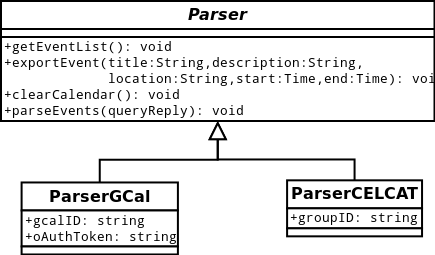
\includegraphics[scale=0.65]{diagclasses_parser.png}
		\caption{Diagramme de classe des interfaces de communication}
	\end{figure}
	\FloatBarrier

\chapter{Conception de l'interface utilisateur}
	%JEROME

